\documentclass[expanded]{lkx_pset}

\title{Math 213b Problem Set 3}
\author{Lev Kruglyak}
\due{February 14, 2024}

\usepackage{graphicx}

\newcommand{\D}{\mathbb{D}}
\newcommand{\x}{\mathbf{x}}
\usepackage{pgfplots}
\pgfplotsset{
	compat=1.12,
}

\newcommand{\dd}{\partial}
\newcommand{\ddc}{\overline{\partial}}

\usepackage{bbm}
\newcommand{\bbDelta}{\bm{\Delta}}


\collaborator{AJ LaMotta}
% \collaborator{Jarell Cheong}

\begin{document}
\maketitle

\begin{problem}{1}
Let $G$ be the finite group of automorphisms of $\CP^{1}$ generated by
$z\mapsto -z$ and $z\mapsto 1/z$. Identify the quotient $\CP^{1}/G$ in
with $\CP^{1}$ in such a way that the quotient map $f: \CP^{1}\to
	\CP^{1}/G \cong \CP^{1}$ is holomorphic, and find the critical points
and critical values of $f$.
\end{problem}

\begin{solution}
	First, note that $G$ is isomorphic to the Klein $4$-group $\Z/2\times \Z/2$.
	Consider the function $f : \CP^1 \to \CP^1$ given by:
	\[
		f(z) = z^2 + \frac{1}{z^2}.
	\]
	Here we can set $f(0)=\infty$ and $f(\infty)=0$ by the Riemann removable singularity theorem. This map is clearly holomorphic as a map between Riemann surfaces. Notice that this map is invariant under the action of $G$, i.e. $f(-z)=f(z)$ and $f(1/z)=f(z)$. Furthermore, since this map has degree $4$, whenever $f(z_1)=f(z_2)$ there must be some $g\in G$ with $z_1 = g\cdot z_2$. This means that $f$ factors uniquely through the quotient, i.e. $f = \varphi \circ \widetilde{f}$ where $\widetilde{f} : \CP^1 \to \CP^1/G$ is the quotient map and $\varphi : \CP^1/G \cong \CP^1$ is a biholomorphism.

	Now let's find the critical points of $f$. The derivative of $f$ is $f'(z) = 2z-2z^{-3}$, and solving $f'(z)=0$ gives us $z^4=1$ and $z=\infty$, so the critical points are the $4$th roots of unity (and infinity). The critical values are then
	\[
		f(\zeta_4^k) = \zeta_4^{2k} + \zeta_4^{-2k} = \frac{\zeta_4^{4k}+1}{\zeta_4^{2k}} = \frac{2}{\zeta_4^{2k}} = \pm 2\quad\textrm{where}\quad \zeta_4=\exp(\pi i/2)
	\]
	and $\infty$. So summarize, the critical points are $\{\pm 1, \pm i, \infty\}$ and the critical values are $\{\pm 2, \infty\}$.
\end{solution}

\begin{problem}{2}
In class, we will prove the
following result: if $X$ is a compact connected Riemann surface of
genus $g$ and $p\in X$ is any point, then there exists a non-constant meromorphic
function $f$ on $X$ that has a pole at $p$ of order at most $g+1$ and
no other poles.
\end{problem}

\begin{parts}
	\begin{part}{}
		Use this to show the following: Given
		distinct points $p_{1},\dots, p_{m}$ in $X$ and any values
		$w_{1},\dots w_{m}$ in $\C$, there exists a meromorphic function $g$
		on $X$ with $f(p_{i})=w_{i}$ for all $i$.
	\end{part}

	Since $X$ is a genus $g$ surface, for any given point $p_i$, we can find some non-constant meromorphic function $g_i$ which has a pole only at $p_i$ of order at most $g+1$. Now let $M$ be some M\"obius transformation which sends $\infty \mapsto 1$. Consider the function
	\[
		f(z) = \sum_{1\leq j \leq m} w_i\cdot \prod_{j\neq i} \frac{M\circ g_i(z)- M\circ g_i(p_j)}{1-M\circ g_i(p_j)}.
	\]
	Letting $f_i$ be the $i$th term in this sum, by construction we know that is a meromorphic function with $f_i(p_i)=w_i$ and $f_i(p_j)=0$ for $j\neq i$. Thus, $f$, which is the sum of these meromorphic functions, satisfies the conditions of the problem.
\end{parts}

\begin{problem}{3}
Use the previous problem and a result from Problem Set 2 to show that
the field of meromorphic functions $\mathcal{M}_{X}$ on a connected
Riemann surface $X$ can be described as a an algebraic extension of
the field of rational functions $\C(z)$ of degree  $d$,
whenever there is a map function $f:X\to \CP^{1}$ of degree $d$.
More generally, $\mathcal{M}_{X}$ is an algebraic extension of
$\mathcal{M}_{Y}$ whenever there is a map $X\to Y$ of degree $d$.
\end{problem}

\begin{solution}
	Let's assume for this problem that $X$ is compact, and $Y$ is a connected Riemann surface, with $f : X \to Y$ a degree $d$ holomorphic map. Now given some regular value $y$ of $f$, we know that $f^{-1}(y) = \{x_1, \ldots, x_d\}$. By the previous problem, given some set of $d$ points $w_i$, we can find some meromorphic function $\xi \in \mathcal{M}_X$ such that $\xi(x_i)=w_i$.

	In particular, we can choose $w_i$ distinct and finite so that $\xi$ satisfies the conditions of Homework 2 Problem 4, which implies that $[\mathcal{M}_X : \mathcal{M}_Y] = d$. When $f$ is a rational function, note that $Y=\CP^1$ so here we get the special case
	\[
		[\mathcal{M}_X, \mathcal{M}_{\CP^1}] = [\mathcal{M}_X, \C(z)] = d.
	\]
\end{solution}

\begin{problem}{4}
Let $S\subset \R^{3}$ be a smooth surface in Euclidean 3-space.
Let $\R^{2}$ have standard Euclidean coordinates $(s,t)$, let
$\Omega\subset \R^{2}$ be open, and let $F:\Omega\to \R^{3}$ be a
smooth injective map parametrizing a little patch $U \subset S$. This
parametrization is called \emph{isothermal} if, at each point $z =(s,t) \in \R^{2}$,
the partial derivatives $F_{s}$ and $F_{t}$ are non-zero orthogonal
vectors of equal length in $\R^{3}$. The coordinates of the inverse map $U\to
	\Omega\subset \R^{2}$ are then referred to as \emph{isothermal coordinates} on the patch $U$ of the surface.
\end{problem}

\begin{parts}
	\begin{part}{}
		Assuming the non-trivial
		result that isothermal coordinates on a surface $S$ exist in the
		neighborhood of any point of $S$, explain, briefly, how we
		can use isothermal coordinates to give $S$ the structure of a Riemann
		surface, as long as it is oriented.
	\end{part}

	Suppose $S$ is a surface with an oriented smooth atlas of isothermic charts. Then transitions maps are smooth diffeomorphisms which preserve angles and orientation, allowing us to consider them as biholomorphisms under some suitable complex structure. Thus, any oriented smooth isothermal atlas is a holomorphic atlas and $S$ can be given the structure of a Riemann surface.

	\begin{part}{}
		Let $S$ be the surface of revolution obtained by rotation the curve
		$y=e^{-x}$ about the $x$ axis. Obtain isothermal
		coordinates $(s,t)$ on $S$, where $s$ is periodic of period $2\pi$.
		Leave your answer as an indefinite integral if you wish, or obtain a
		closed form. Beware that if you use Mathematica, as I did, to evaluate
		the integral then you will run into Mathematica's weakness for
		yielding answers that don't really make sense for real variables.
	\end{part}

	Let $x(t) : I \to \R$ be a smooth function on an open interval $I$. Then consider the map $F : \Omega \to \R^3$ on $\Omega=(\theta,\theta+2\pi)\times I$ for $\theta\in \R$ given by
	\[
		F(s,t)=(x(t), e^{-x(t)}\cos(s), e^{-x(t)}\sin(s)).
	\]
	We would like to show that some subset of this family of maps consists of isothermal maps, i.e. we have
	\[
		\frac{\partial F}{\partial s}\cdot \frac{\partial F}{\partial t} = 0,\quad \textrm{and}\quad \left|\frac{\partial F}{\partial s}\right|^2=\left|\frac{\partial F}{\partial t}\right|.
	\]
	Expanding out the partials, we have
	\[
		\begin{aligned}
			\frac{\partial F}{\partial s}(s,t) & = (0, -e^{-x(t)}\sin(s), e^{-x(t)}\cos(s)),                \\
			\frac{\partial F}{\partial t}(s,t) & = (x'(t), -x'(t)e^{-x(t)}\cos(s), -x'(t)e^{-x(t)}\sin(s)),
		\end{aligned}
	\]
	so clearly the orthogonality condition is satisfied. For the second condition to be satisfied, we require that
	\[
		e^{-2x(t)} = x'(t)^2(1+e^{-2x(t)}) \quad\implies\quad x'(t) = \sqrt{\frac{1}{1+e^{2x(t)}}}.
	\]
	We can thus choose $x(t)$ to be strictly increasing. Solving the differential equation in this case, we observe that the inverse of $x(t)$ has the form
	\[
		x^{-1}(t) = \int_0^t \sqrt{1+e^{2x}}\,dx
	\]
	This completes the proof that $S$ admits isothermal coordinates.
\end{parts}

\begin{problem}{5}
Let $C\subset \C^{2}$ be the Riemann surface defined by the
equation $w^{2}=z(z+4)(z-2)$ (a non-compact Riemann surface).
Sketch this locus in the real plane (i.e. for $(z,w) \in \R^{2}$).
Show that the curve $C$ carries a meromorphic function with
\begin{itemize}
	\item a simple zero at $(z,w)=(-1,3)$,
	\item a simple pole at
	      $(z,w)=(-1,-3)$,
	\item one other simple zero somewhere,
	\item no other zeros or poles.
\end{itemize}
Find the coordinates of the other zero.

% \emph{Hint.} Thinking about the tangent line to the curve at
% $(-1,3)$ will help.
\end{problem}

\begin{solution}
	Here is a sketch of the intersection of $C$ with the real plane:
	\begin{center}
		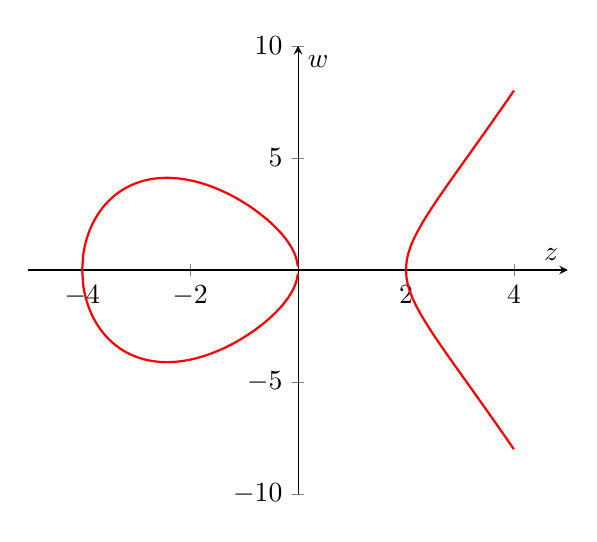
\begin{tikzpicture}
			\begin{axis}[
					xmin=-5, xmax=5, ymin=-10, ymax=10, xlabel={$z$}, ylabel={$w$},
					axis lines=middle, samples=200, smooth, clip=false,
				]
				\addplot [red, thick, domain=-4:0.1] {sqrt(x*(x+4)*(x-2))};
				\addplot [red, thick, domain=-4:0.1] {-sqrt(x*(x+4)*(x-2))};
				\addplot [red, thick, domain=2:4] {sqrt(x*(x+4)*(x-2))};
				\addplot [red, thick, domain=2:4] {-sqrt(x*(x+4)*(x-2))};
			\end{axis}
		\end{tikzpicture}
	\end{center}
	Let's investigate this function by thinking about the tangent line to the curve. By implicit differentiation, we have the relation
	\[
		2w\cdot \frac{\partial w}{\partial z} = 3z^2 + 4z - 8.
	\]
	At $(z,w)=(-1,3)$, the slope of the tangent line to $C$ is then $-3/2$. Thus, the equation for the tangent line $L$ at this point is
	$3(z+1)+2(w-3)=0.$ Plugging this into the defining polynomial for $C$, we get
	\[
		w^2 - z(z+4)(z-2) = -\frac{1}{4}(z+1)^2 (4z-9) = 0.
	\]
	This polynomial has a zero of order $2$ at $z=-1$, which corresponds to $w=3$, and a zero of order $1$ at $z=9/4$, corresponding to $w=-15/8$. Consider now the line $z=-1$, which intersects $C$ at $(-1,3)$ and $(-1,-3)$, each with multiplicity $1$. Taking the ratio of these two lines then gives the desired meromorphic function, since
	\[
		f(z) = \frac{3(z+1)+2(w-3)}{z+1}
	\]
	has simple zeroes at $(-1,3)$ and $(9/4, -15/8)$, and a simple pole at $(-1,-3)$, with no other zeroes or poles.
\end{solution}

\end{document}
